%!TEX root=../template.tex


Since DRAM has low-density, DRAM-based memory system may contribute as much as 40\% in the total processor power. The power consumed by processor includes power of processor cores, L1, L2 and L3 caches, cache controllers, and cache directories. The power consumed by memory includes the power consumption of DRAM memory, memory controllers, and peripheral circuit such as row buffer and sense amplifier. We can see that not only DRAM itself will consume lots of power, but its peripheral component will also consume large portion of overall power. Researchers have tried to minimize power consumption of traditional memory system with performance-optimized design and optimized power-management techniques. It is clear that traditional memory system may consume very large amount of power in commercial processors. What's more, the process scaling of DRAM to smaller feature size has become more and more challenging.   


\subsection{PCM }
\label{sec:backgrouond:PCM}


PCM ~\cite{5609179}is an emerging memory technology, which has recently received a lot of attention. PCM is a emerging non-volatile memory which can contain data for over 10 years with high retention property and very good operation characteristics and scalability as shown in ~\Fig{fig:sttpcm cell}. PCM has high storage density and PCM prototypes with feature size as small as 3nm have been fabricated and it also has higher write endurance than the flash memory. PCM with little leakage power has almost the same read power and latency compared with DRAM. However, PCM has worse write endurance than that of DRAM, also its write power is significantly higher than that of DRAM. Writing to a PCM cell requires high current density for a large period of time. Thus, it is forced to limit the number of simultaneous writes to ensure correct operation, which will limit write throughput and overall performance of PCM. Thus, failure to save write energy may counteract the power saving advantage gained due to low leakage power.  

The emerging PCM technology has many advantages compared with DRAM such as non-volatility, low leakage power, scalability and fast read cycle. Different from DRAM storing data using capacity, PCM uses the differences between the two states in the electrical resistivity of GST to store information. The GST phase can be changed using electrical-pulse generated Joule heat by heating a region of phase change material to very high temperature, which will lead to high write energy and long latency compared with DRAM.       



%\begin{figure}[t!]
\begin{figure}[t]
\centering
% 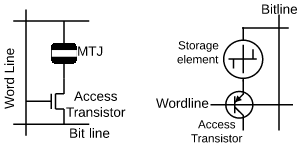
\includegraphics[scale=0.7]{figs/sttt-pcm}
 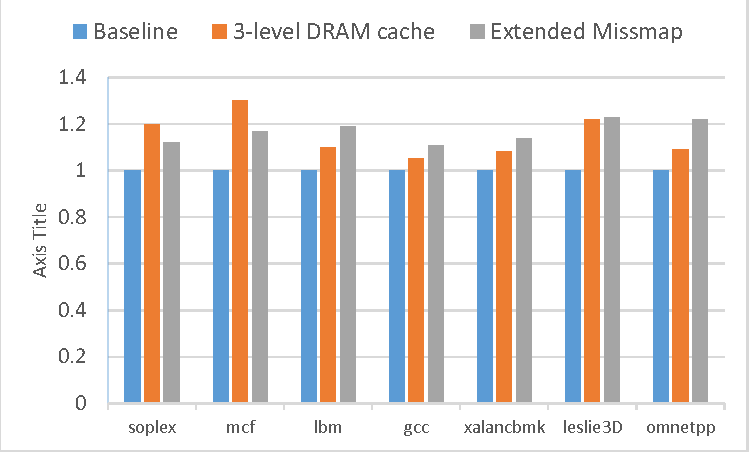
\includegraphics[scale=0.7]{figs/vector}    

%\includegraphics[trim=0 0 0 0, clip, width=\columnwidth]{figs/browser-arch}
\caption{Basic Cell of STT-RAM and PCM.}
\label{fig:sttpcm cell}
\end{figure}


A PCM cell is consisted of an NMOS access transistor and a storage resistor. To store a binary data on PCM, heat is applied to the cell which transitions the physical state of the storage resistor with particular resistances. When the resistor is heated to a very high temperature and quickly cooled down, it transits into an amorphous substance with high electrical resistance which represents binary “0”. On the other hand, it can also change to a physical state with lower resistance, which represents binary “1”.    

%It is clear that while DRAM stores data as a small amount of electric charge in a capacitor, the PCM’s approach to storing data is fundamentally different. This difference gives PCM the potential for better technology scaling, leading to higher density, lower cost per bit, and larger capacity memory than DRAM. The difference in resistance values between the two states of PCM is typically 3 orders of magnitude. PCM memories achieve high density by exploiting this high resistance range to store multiple bits in a single cell, this structure is known as multi-level cell or MLC.




\subsection{STT-RAM}
\label{sec:background:stt-ram}



\begin{comment}

\begin{table}[t]
\caption{\small Requirements met by common benchmarks.}
\renewcommand{\arraystretch}{.95}                                                   
\resizebox{\columnwidth}{!}{
\centering
\begin{tabular}{|c|c|c|c|c|}
\hline
&Popular&Representative&Diverse&Repeatible \\ \hline
Realistic Webpage & \checkmark & \checkmark & \checkmark & X \\ \hline
BBench & \checkmark & ? & ? & \checkmark \\ \hline
BrowsingBench & X & X & ? & \checkmark \\ \hline
Zhu et. al & \checkmark & ? & ? & \checkmark \\ \hline
\end{tabular}
}
\label{tab:requirements}
\end{table}


\end{comment}


Spin-Transfer Torque Random Access Memory (STT-RAM) cell is consisted of a transistor and magnetic tunnel junction (MTJ) as shown in ~\Fig{fig:sttpcm cell} ~\cite{aware}. In an STT-RAM cell, data is stored using two or more resistance states of a magnetic tunneling junction (MTJ) device. The MTJ is consisted of a pinned and a free magnetic layer separated by a tunneling oxide barrier. The magnetization of the pinned layer (PL) is fixed whereas that of the free layer (FL) can be changed by using an electrical current. The FL magnetization is stable in two states such that in one state it is parallel to the magnetization of the PL, whereas in the other state it is antiparallel to PL. The MTJ exhibits a different resistance based on whether the magnetization of the two magnetic layers is in parallel (P) or antiparallel (AP) configuration. In the P state, resistance of the MTJ is low representing a logical “1”. In AP state, the resistance of the MTJ is high representing a logical “0”. Because of its nonvolatile nature there is no leakage in STT-RAM cells when they are not accessed. Therefore, STT-RAM has been investigated as candidate for replacing SRAM in the last level cache (LLC) or replacing DRAM in memory. Due to low utilization of LLC and frequent refresh of DRAM, the leakage in memory bit-cells in the dominant component of the total energy consumption. Thus, STT-RAM based memory is expected to significantly lower total energy consumption by eliminating leakage power.  


In spite of these advantages,  there are two major obstacles to use STT-RAM for on-chip LLC and memory, namely, its longer write latency and higher write energy. During a STT-RAM write operation, the MTJ resistance switching mechanism is dominated by time. The required switching current increases exponentially as MTJ switching time is reduced ~\cite{xu}. The corresponding transistor’s size must increase accordingly, leading to a larger memory cell area. The lifetime of memory cell may also degrades due to increasing voltage across the MTJ. Therefore, 10ns switching time of write operation is the design limit for further performance optimization.  



\subsection{NVM optimization}
\label{sec:background:optimization}

To meet the demands of power-budget of NVM computer system, low power management techniques have been proposed for all range of computing systems ranging from embedded system to supercomputer. There are many techniques are proposed to optimize NVM. One of these techniques is to convert NVM write operation to read-before-write operation to reduce write energy. Some other techniques are reducing unnecessary write back from row buffer to NVM main memory. Some researchers propose last level cache management techniques for improving energy efficiency of NVM main memory. Some researchers have proposed compression based techniques to reduce write-traffic to NVM. Several other techniques aim to address the write latency issue, and its harmful impact on read latency arising due to bank conflicts and try to utilize write locality to coalesce all possible changes to the data by using buffers before they are finally written to NVM. 


\subsubsection{Minimizing NVM Main Memory Power by Managing Caches}
In the memory hierarchy of modern processors, main memory and caches exist close to each other and thus, intelligent management of caches can translate into optimization of performance and energy efficiency at main memory. The design goal of these techniques is to minimize cache miss-rate and/or writebacks to reduce the accesses to memory, which leads to saving in energy of memory. Some researchers propose a cache replacement policy for saving NVM main memory energy. Their approach aims to reduce the write-back traffic to main memory. Some researchers proposed a technique to reduce the number of writebacks from LLC to NVM main memory for reducing the power consumption of NVM memory. Other researchers used a design space exploration approach for finding the optimal configuration of cache hierarchy in a system with non-volatile memory.


Last-level cache (LLC) organizations offer trade-offs between on-chip data locality and off-chip miss rate. While private LLC organizations have low hit latencies, their off-chip miss rates are high in applications that have uneven distributions of working sets or exhibit high degrees of sharing (due to cache line replication). On the other hand, shared LLC organizations have low off-chip miss rates since cache lines are not replicated.

\subsubsection{Reducing NVM Write Traffic} 
As discussed before, the write latency and energy of NVM are significantly higher than that of DRAM. Reducing number can greatly reduce the number of writes to NVM memory. The reduction in write-traffic improves the performance and also reduces the dynamic energy of NVM main memory. Redundant writes may be avoided by either actual comparison with originally stored data, or using flags which track whether the portions of the data being written have actually changed and then writing only the changed data-words.Some researchers proposed a technique for reducing the number of writes to NVM main memory based on data migration and re-computation ~\cite{6844484}. Some researchers proposed a register-allocation based technique with re-computation to reduce the number of store instructions to non-volatile memory.

There is observation that a large fraction of words in a cache line being written back to memory are not actually modified. Our technique based on the observation that there is huge clean cache write back of gem5 based existing cache coherence policy changing from state Modify to Invalid through MI state. 


\begin{figure}[t]
\centering
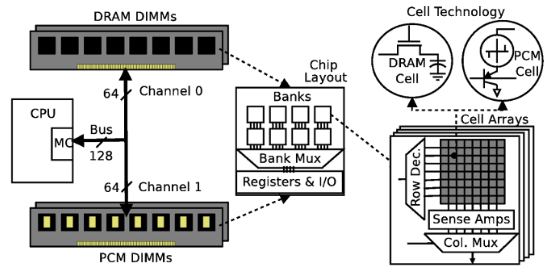
\includegraphics[width=\columnwidth]{figs/hybrid}
%\includegraphics[trim=0 0 0 0, clip, width=\columnwidth]{figs/browser-arch}
\caption{Hybrid Memory System with DRAM and PCM.}
\label{fig:hybrid}
\end{figure}






\subsubsection{Hybrid NVM-DRAM Architecture}
NVM-DRAM hybrid main memory system architectures, as shown in ~\Fig{fig:hybrid}, aim to utilize the best features of different technologies, such as performance, cost, energy, reliability, endurance. There are many research in this direction, some people proposed a hybrid memory design where NVM memory is augmented with a small DRAM that acts as a “page cache” for the NVM memory. The page cache buffers frequently accessed pages and thus helps performance and improves NVM endurance by reducing the number of writes to NVM with write combining and coalescing. Some researchers proposed a memory management technique for hybrid NVM-DRAM memory to hide the slow write performance of NVM. Some researchers proposed a migration based page caching technique for NVM-DRAM hybrid main memory system. Their technique aims to overcome the problem of the long latency and low endurance of NVM.    



\subsubsection{Cache Replacement Policy}
Most existing work on DRAM-based main memory systems mainly concentrates on improving cache read hit ratio since dirty pages will be flushed back to storage quite frequently. Belady’s optimal page replacement policy leads to the optimal cache hit ratio. This algorithm always discards pages that will not be needed for the longest time in the future. To predict a page’s future access pattern, recency and frequency are two valuable indicators. Some of the existing work, such as Least Recently Used (LRU) and Least Frequently Used (LFU). The traditional LRU policy is not suitable in the hybrid memory architecture, because the penalty write back to DRAM and NVM is different, so some researchers improved cache replacement policy by adding additional tag to cache to determine the cache block coming from DRAM or NVM. When cache miss happens, the tag is used to decide different penalty or replacement policy.    





\subsection{Simulator}
Simulation frameworks have always been a powerful tool in the hands of computer architects. Incorporating detailed performance models in simulators and using them to approximate the behavior of real hardware enables the computer designers to experiment with a variety of different configurations early in the design stage of a system and investigate interesting trade- offs before the prototype stage of the design process. 
In this report, we primarily use gem5, which is a system simulator built from a combination of M5 and GEMS simulators. gem5 supports most commercial ISAs such as x86, ARM, and MIPS. It can run a full system simulation and provide a cycle based model for out-of-order processors and gives the designer a better insight and can prove an extremely useful tool. It can help use to gain insight about how real hardware works with respect to application behavior without actual access the physical hardware. Memory hierarchy organization, pipeline design and interconnection between multiple cores are primarily design interest of computer architect.   












